%% bare_conf.tex
%% V1.4b
%% 2015/08/26
%% by Michael Shell
%% See:
%% http://www.michaelshell.org/
%% for current contact information.
%%
%% This is a skeleton file demonstrating the use of IEEEtran.cls
%% (requires IEEEtran.cls version 1.8b or later) with an IEEE
%% conference paper.
%%
%% Support sites:
%% http://www.michaelshell.org/tex/ieeetran/
%% http://www.ctan.org/pkg/ieeetran
%% and
%% http://www.ieee.org/

%%*************************************************************************
%% Legal Notice:
%% This code is offered as-is without any warranty either expressed or
%% implied; without even the implied warranty of MERCHANTABILITY or
%% FITNESS FOR A PARTICULAR PURPOSE! 
%% User assumes all risk.
%% In no event shall the IEEE or any contributor to this code be liable for
%% any damages or losses, including, but not limited to, incidental,
%% consequential, or any other damages, resulting from the use or misuse
%% of any information contained here.
%%
%% All comments are the opinions of their respective authors and are not
%% necessarily endorsed by the IEEE.
%%
%% This work is distributed under the LaTeX Project Public License (LPPL)
%% ( http://www.latex-project.org/ ) version 1.3, and may be freely used,
%% distributed and modified. A copy of the LPPL, version 1.3, is included
%% in the base LaTeX documentation of all distributions of LaTeX released
%% 2003/12/01 or later.
%% Retain all contribution notices and credits.
%% ** Modified files should be clearly indicated as such, including  **
%% ** renaming them and changing author support contact information. **
%%*************************************************************************


% *** Authors should verify (and, if needed, correct) their LaTeX system  ***
% *** with the testflow diagnostic prior to trusting their LaTeX platform ***
% *** with production work. The IEEE's font choices and paper sizes can   ***
% *** trigger bugs that do not appear when using other class files.       ***                          ***
% The testflow support page is at:
% http://www.michaelshell.org/tex/testflow/



\documentclass[conference]{IEEEtran}

\usepackage{cite}
\usepackage[T1]{fontenc}
\usepackage[utf8]{inputenc}
\usepackage{amsfonts}
\usepackage{graphicx}
\usepackage{amsmath}
% Some Computer Society conferences also require the compsoc mode option,
% but others use the standard conference format.
%
% If IEEEtran.cls has not been installed into the LaTeX system files,
% manually specify the path to it like:
% \documentclass[conference]{../sty/IEEEtran}





% Some very useful LaTeX packages include:
% (uncomment the ones you want to load)


% *** MISC UTILITY PACKAGES ***
%
%\usepackage{ifpdf}
% Heiko Oberdiek's ifpdf.sty is very useful if you need conditional
% compilation based on whether the output is pdf or dvi.
% usage:
% \ifpdf
%   % pdf code
% \else
%   % dvi code
% \fi
% The latest version of ifpdf.sty can be obtained from:
% http://www.ctan.org/pkg/ifpdf
% Also, note that IEEEtran.cls V1.7 and later provides a builtin
% \ifCLASSINFOpdf conditional that works the same way.
% When switching from latex to pdflatex and vice-versa, the compiler may
% have to be run twice to clear warning/error messages.






% *** CITATION PACKAGES ***
%
%\usepackage{cite}
% cite.sty was written by Donald Arseneau
% V1.6 and later of IEEEtran pre-defines the format of the cite.sty package
% \cite{} output to follow that of the IEEE. Loading the cite package will
% result in citation numbers being automatically sorted and properly
% "compressed/ranged". e.g., [1], [9], [2], [7], [5], [6] without using
% cite.sty will become [1], [2], [5]--[7], [9] using cite.sty. cite.sty's
% \cite will automatically add leading space, if needed. Use cite.sty's
% noadjust option (cite.sty V3.8 and later) if you want to turn this off
% such as if a citation ever needs to be enclosed in parenthesis.
% cite.sty is already installed on most LaTeX systems. Be sure and use
% version 5.0 (2009-03-20) and later if using hyperref.sty.
% The latest version can be obtained at:
% http://www.ctan.org/pkg/cite
% The documentation is contained in the cite.sty file itself.






% *** GRAPHICS RELATED PACKAGES ***
%
\ifCLASSINFOpdf
% \usepackage[pdftex]{graphicx}
% declare the path(s) where your graphic files are
% \graphicspath{{../pdf/}{../jpeg/}}
% and their extensions so you won't have to specify these with
% every instance of \includegraphics
% \DeclareGraphicsExtensions{.pdf,.jpeg,.png}
\else
% or other class option (dvipsone, dvipdf, if not using dvips). graphicx
% will default to the driver specified in the system graphics.cfg if no
% driver is specified.
% \usepackage[dvips]{graphicx}
% declare the path(s) where your graphic files are
% \graphicspath{{../eps/}}
% and their extensions so you won't have to specify these with
% every instance of \includegraphics
% \DeclareGraphicsExtensions{.eps}
\fi
% graphicx was written by David Carlisle and Sebastian Rahtz. It is
% required if you want graphics, photos, etc. graphicx.sty is already
% installed on most LaTeX systems. The latest version and documentation
% can be obtained at: 
% http://www.ctan.org/pkg/graphicx
% Another good source of documentation is "Using Imported Graphics in
% LaTeX2e" by Keith Reckdahl which can be found at:
% http://www.ctan.org/pkg/epslatex
%
% latex, and pdflatex in dvi mode, support graphics in encapsulated
% postscript (.eps) format. pdflatex in pdf mode supports graphics
% in .pdf, .jpeg, .png and .mps (metapost) formats. Users should ensure
% that all non-photo figures use a vector format (.eps, .pdf, .mps) and
% not a bitmapped formats (.jpeg, .png). The IEEE frowns on bitmapped formats
% which can result in "jaggedy"/blurry rendering of lines and letters as
% well as large increases in file sizes.
%
% You can find documentation about the pdfTeX application at:
% http://www.tug.org/applications/pdftex





% *** MATH PACKAGES ***
%
%\usepackage{amsmath}
% A popular package from the American Mathematical Society that provides
% many useful and powerful commands for dealing with mathematics.
%
% Note that the amsmath package sets \interdisplaylinepenalty to 10000
% thus preventing page breaks from occurring within multiline equations. Use:
%\interdisplaylinepenalty=2500
% after loading amsmath to restore such page breaks as IEEEtran.cls normally
% does. amsmath.sty is already installed on most LaTeX systems. The latest
% version and documentation can be obtained at:
% http://www.ctan.org/pkg/amsmath





% *** SPECIALIZED LIST PACKAGES ***
%
%\usepackage{algorithmic}
% algorithmic.sty was written by Peter Williams and Rogerio Brito.
% This package provides an algorithmic environment fo describing algorithms.
% You can use the algorithmic environment in-text or within a figure
% environment to provide for a floating algorithm. Do NOT use the algorithm
% floating environment provided by algorithm.sty (by the same authors) or
% algorithm2e.sty (by Christophe Fiorio) as the IEEE does not use dedicated
% algorithm float types and packages that provide these will not provide
% correct IEEE style captions. The latest version and documentation of
% algorithmic.sty can be obtained at:
% http://www.ctan.org/pkg/algorithms
% Also of interest may be the (relatively newer and more customizable)
% algorithmicx.sty package by Szasz Janos:
% http://www.ctan.org/pkg/algorithmicx




% *** ALIGNMENT PACKAGES ***
%
%\usepackage{array}
% Frank Mittelbach's and David Carlisle's array.sty patches and improves
% the standard LaTeX2e array and tabular environments to provide better
% appearance and additional user controls. As the default LaTeX2e table
% generation code is lacking to the point of almost being broken with
% respect to the quality of the end results, all users are strongly
% advised to use an enhanced (at the very least that provided by array.sty)
% set of table tools. array.sty is already installed on most systems. The
% latest version and documentation can be obtained at:
% http://www.ctan.org/pkg/array


% IEEEtran contains the IEEEeqnarray family of commands that can be used to
% generate multiline equations as well as matrices, tables, etc., of high
% quality.




% *** SUBFIGURE PACKAGES ***
%\ifCLASSOPTIONcompsoc
%  \usepackage[caption=false,font=normalsize,labelfont=sf,textfont=sf]{subfig}
%\else
%  \usepackage[caption=false,font=footnotesize]{subfig}
%\fi
% subfig.sty, written by Steven Douglas Cochran, is the modern replacement
% for subfigure.sty, the latter of which is no longer maintained and is
% incompatible with some LaTeX packages including fixltx2e. However,
% subfig.sty requires and automatically loads Axel Sommerfeldt's caption.sty
% which will override IEEEtran.cls' handling of captions and this will result
% in non-IEEE style figure/table captions. To prevent this problem, be sure
% and invoke subfig.sty's "caption=false" package option (available since
% subfig.sty version 1.3, 2005/06/28) as this is will preserve IEEEtran.cls
% handling of captions.
% Note that the Computer Society format requires a larger sans serif font
% than the serif footnote size font used in traditional IEEE formatting
% and thus the need to invoke different subfig.sty package options depending
% on whether compsoc mode has been enabled.
%
% The latest version and documentation of subfig.sty can be obtained at:
% http://www.ctan.org/pkg/subfig




% *** FLOAT PACKAGES ***
%
%\usepackage{fixltx2e}
% fixltx2e, the successor to the earlier fix2col.sty, was written by
% Frank Mittelbach and David Carlisle. This package corrects a few problems
% in the LaTeX2e kernel, the most notable of which is that in current
% LaTeX2e releases, the ordering of single and double column floats is not
% guaranteed to be preserved. Thus, an unpatched LaTeX2e can allow a
% single column figure to be placed prior to an earlier double column
% figure.
% Be aware that LaTeX2e kernels dated 2015 and later have fixltx2e.sty's
% corrections already built into the system in which case a warning will
% be issued if an attempt is made to load fixltx2e.sty as it is no longer
% needed.
% The latest version and documentation can be found at:
% http://www.ctan.org/pkg/fixltx2e


%\usepackage{stfloats}
% stfloats.sty was written by Sigitas Tolusis. This package gives LaTeX2e
% the ability to do double column floats at the bottom of the page as well
% as the top. (e.g., "\begin{figure*}[!b]" is not normally possible in
% LaTeX2e). It also provides a command:
%\fnbelowfloat
% to enable the placement of footnotes below bottom floats (the standard
% LaTeX2e kernel puts them above bottom floats). This is an invasive package
% which rewrites many portions of the LaTeX2e float routines. It may not work
% with other packages that modify the LaTeX2e float routines. The latest
% version and documentation can be obtained at:
% http://www.ctan.org/pkg/stfloats
% Do not use the stfloats baselinefloat ability as the IEEE does not allow
% \baselineskip to stretch. Authors submitting work to the IEEE should note
% that the IEEE rarely uses double column equations and that authors should try
% to avoid such use. Do not be tempted to use the cuted.sty or midfloat.sty
% packages (also by Sigitas Tolusis) as the IEEE does not format its papers in
% such ways.
% Do not attempt to use stfloats with fixltx2e as they are incompatible.
% Instead, use Morten Hogholm'a dblfloatfix which combines the features
% of both fixltx2e and stfloats:
%
% \usepackage{dblfloatfix}
% The latest version can be found at:
% http://www.ctan.org/pkg/dblfloatfix




% *** PDF, URL AND HYPERLINK PACKAGES ***
%
%\usepackage{url}
% url.sty was written by Donald Arseneau. It provides better support for
% handling and breaking URLs. url.sty is already installed on most LaTeX
% systems. The latest version and documentation can be obtained at:
% http://www.ctan.org/pkg/url
% Basically, \url{my_url_here}.




% *** Do not adjust lengths that control margins, column widths, etc. ***
% *** Do not use packages that alter fonts (such as pslatex).         ***
% There should be no need to do such things with IEEEtran.cls V1.6 and later.
% (Unless specifically asked to do so by the journal or conference you plan
% to submit to, of course. )


% correct bad hyphenation here
\hyphenation{op-tical net-works semi-conduc-tor}


\begin{document}
    %
    % paper title
    % Titles are generally capitalized except for words such as a, an, and, as,
    % at, but, by, for, in, nor, of, on, or, the, to and up, which are usually
    % not capitalized unless they are the first or last word of the title.
    % Linebreaks \\ can be used within to get better formatting as desired.
    % Do not put math or special symbols in the title.
    \title{Proseminar \\Hardwareimplementations of Artifical Neural Networks}


    % author names and affiliations
    % use a multiple column layout for up to three different
    % affiliations
    \author{
    \IEEEauthorblockN{Leon Jungemeyer}
    \IEEEauthorblockA{
    Department of Informatics\\
    Karlsruhe Institute of Technology\\
    Karlsruhe, Germany\\
    Email: leon.jungemeyer@me.com
    }
    }

    % conference papers do not typically use \thanks and this command
    % is locked out in conference mode. If really needed, such as for
    % the acknowledgment of grants, issue a \IEEEoverridecommandlockouts
    % after \documentclass

    % for over three affiliations, or if they all won't fit within the width
    % of the page, use this alternative format:
    %
    %\author{\IEEEauthorblockN{Michael Shell\IEEEauthorrefmark{1},
    %Homer Simpson\IEEEauthorrefmark{2},
    %James Kirk\IEEEauthorrefmark{3},
    %Montgomery Scott\IEEEauthorrefmark{3} and
    %Eldon Tyrell\IEEEauthorrefmark{4}}
    %\IEEEauthorblockA{\IEEEauthorrefmark{1}School of Electrical and Computer Engineering\\
    %Georgia Institute of Technology,
    %Atlanta, Georgia 30332--0250\\ Email: see http://www.michaelshell.org/contact.html}
    %\IEEEauthorblockA{\IEEEauthorrefmark{2}Twentieth Century Fox, Springfield, USA\\
    %Email: homer@thesimpsons.com}
    %\IEEEauthorblockA{\IEEEauthorrefmark{3}Starfleet Academy, San Francisco, California 96678-2391\\
    %Telephone: (800) 555--1212, Fax: (888) 555--1212}
    %\IEEEauthorblockA{\IEEEauthorrefmark{4}Tyrell Inc., 123 Replicant Street, Los Angeles, California 90210--4321}}




    % use for special paper notices
    %\IEEEspecialpapernotice{(Invited Paper)}




    % make the title area
    \maketitle

    % As a general rule, do not put math, special symbols or citations
    % in the abstract
    \begin{abstract}
        The inherent parallel nature of neural networks makes software implementations of Neural Networks perform poorly on classic
        von-Neumann architectures.
        This is why different types of hardware accelerators aim to improve performance of neural computation.

        This paper presents an overview of recent approaches to implement Artificial Neural Networks(ANN) directly into hardware.
        Specifically, analog versus digital implementations of ANNs are compared by there respective advantages and disadvantages.
        Furthermore, we take a look into the future of neural processing units and recent research around ANN implementations using memristors.
    \end{abstract}

    % no keywords




    % For peer review papers, you can put extra information on the cover
    % page as needed:
    % \ifCLASSOPTIONpeerreview
    % \begin{center} \bfseries EDICS Category: 3-BBND \end{center}
    % \fi
    %
    % For peerreview papers, this IEEEtran command inserts a page break and
    % creates the second title. It will be ignored for other modes.
    \IEEEpeerreviewmaketitle



    \section{Introduction}

    Artificial neural networks are a biologically inspired concept in computer science, to classify and process large amounts of data.
    Originally, ANNs were a concept designed in software and computed on classic processors.
    Because of the massive amount of parallel operations, classic processors struggle to keep up with modern requirements to neural networks \cite{forssell2014hardware}.
    Hardwareimplementations of ANNs try to solve that problem by designing a processing architecture tailored directly to ANNs.

    ANNs are used in a variety of applications.
    Each applications has different requirements to the neural networks used.
    Requirements can vary between computing speed, the topography of the neural network, the required precision and many more.
    Similar to classic processors, this calls for a highly flexible architecture that can be adapted to fit the need of the respective application.

    In addition to classifying data, learning is a key element of neural networks.
    However, not every application requires on chip learning.
    Especially in consumer products, pre-trained networks with no need for later training might be shipped.

    Since learning requires a lot of additional hardware, some ANN implementations sacrifice on chip learning to allow for a less complex and expensive hardware.


    \section{Artificial Neurons}

    Neurons are the basic building blocks for any ANN.
    Hardwareimplementations differ substantially between analog and digital implementations, and also between activation functions(AF) \cite{habib1989digital}.

    A single neuron applies an activation function to the weighed sum over all its inputs.

    \[y = f(\sum_i {w_ix_i} + b)\]

    The activation function(AF) is typically a nonlinear function that maps its input into a range between 0 and 1.

    \[ f: \mathbb{R} \to [0,1] \subset \mathbb{R} \]

    \begin{figure}[h]
        \centering
        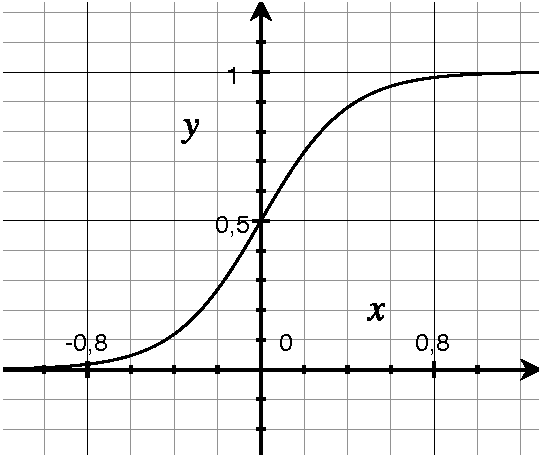
\includegraphics[width=0.25\textwidth]{resources/sigmoid.pdf}
        \caption{An example sigmoid activation function. $y = \frac{1}{1+e^{-5x}}$}
        \label{fig:sigmoid}
    \end{figure}

    In \ref{fig:neuron} the structure of a neuron is illustrated.

    \begin{figure}[h]
        \centering
        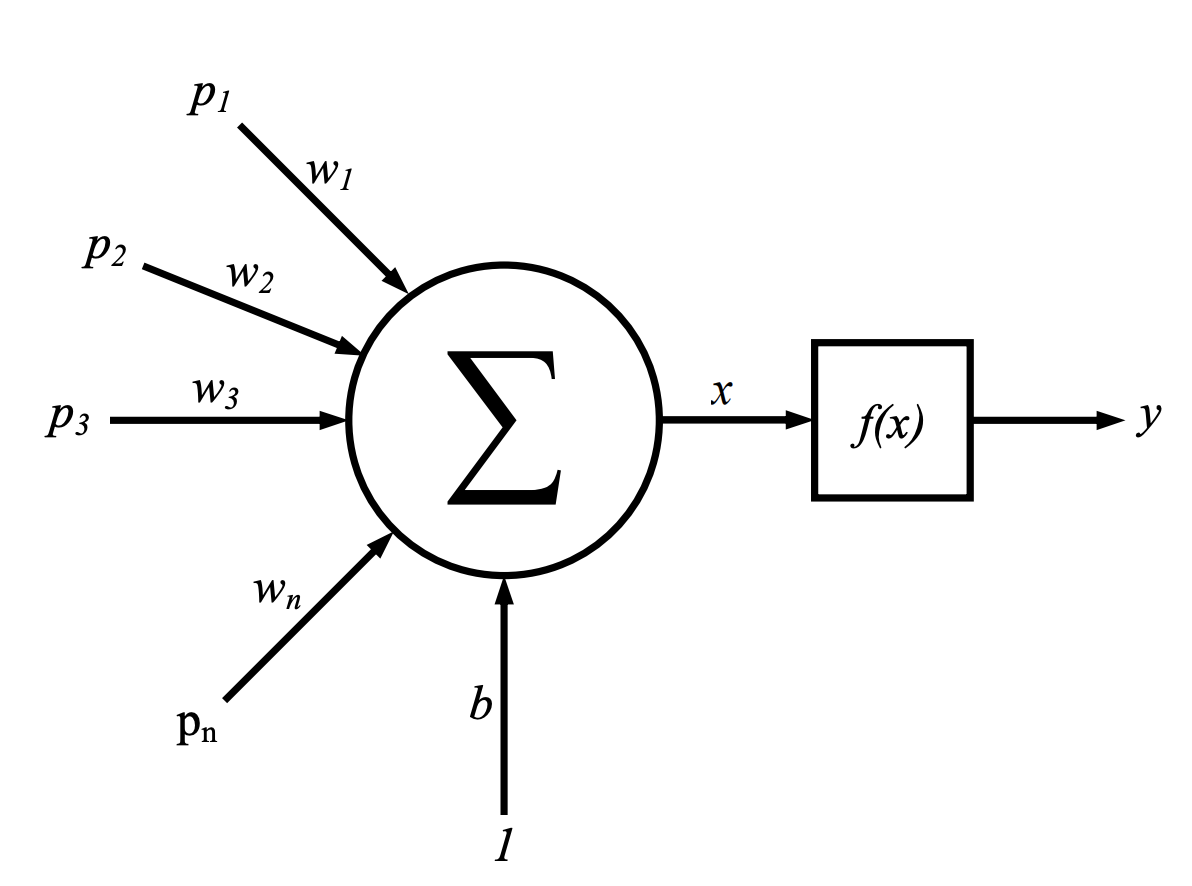
\includegraphics[width=0.25\textwidth]{resources/neuron.png}
        \caption{A single neuron with synapse weights $w_1,\dots,w_n$, bias $b$ and AF $f(x)$, as illustrated in \cite[Fig.~1]{muthuramalingam2008neural}.}
        \label{fig:neuron}
    \end{figure}


    \subsection{Digitale Neuronen}

    Aufgrund der weiten Verbreitung von CMOS Technologie sind digitale Implementierungen von künstlichen Neuronen relativ günstig umzusetzen\cite{misra2010artificial} .

    \subsubsection{FPGA Basierte Implementierungen}
    In \cite{muthuramalingam2008neural} wird eine implemntierung eines Neurons mittles eines FPGAs Vorgeschlagen.
    Dabei wird das Neuron in 2 Teile unterteilt, des sogentannten \texttt{SIGMA} Block und den \texttt{LOGSIG} Block.

    Der \texttt{SIGMA} Block berechnet dabei die gewichtete Summe der Eingangswerte plus den Bias.

    Der \texttt{LOGSIG} Block übernimmt dann das berechnen der Aktivierungsfunktion.
    Als Aktivierungsfunktion wird hier $f(x) = \frac{1}{1+e^{-x}}$ verwendet.

    Eine weitere Möglichkeit besteht darin, anstelle einer Berechnung der Aktivierungsfunktion eine Look UP Tabelle (LUT) zu verwenden.
    Die LUT wird direkt im RAM des Neurons gespeichert.
    Dabei muss beachtet werden, das die größe der LUT die Genauigkeit der Aktivierungsfunktion bestimmt.
    Durch Verwendung einer LUT kann sowohl der Energieverbrauch als auch die Rechenzeit deutlich reduziert werden \cite{muthuramalingam2008neural} .


    \subsection{Analoge Neuronen}

    Wie digitale Neuronen bilden auch analoge Neuronen die gewichtete Summe über ihre Eingaben.
    Um die Gewichte der Synapsen zu modlieren gibt es veschiedene Ansätze.

    \subsubsection{Gewichtete Summe}
    In einfachen Implementiereungen kann man Widerstände als Gewichte verwenden \cite{zurada1992analog} .
    Diese können dann mithilfe eines Spannungsaddierers(Summing Amplifier) addiert werden.
    Die Ausgangssspannung ist dann gerade die Summe der Gewichte.

    %TODO: Add Fig. 1 von zurada1992analog

    \subsubsection{Aktivierungsfunktion}
    Die einfachste Aktivierungsfunktion ist digital wie auch analog die Identitätsfunktion.
    Durch Anpassen der Gewichte kann diese linear Skaliert werden. \cite{zurada1992analog}


    \subsubsection{Synapsen}
    Das Hauptproblem analoger ANNs besteht darin, anpassbare Gewichte für Synapsen zu implementieren.

    Gewichte können dabei über Varaible wiederstände simuliert werden, welche anhand der angelegten Spannung auf den richtigen Wiederstand gebracht werden.
    Die Gewichte bzw die angelegte Spannung muss dann gespeichtert werden.

    %TODO: Resistor: Siehe VLSI implementation of a neural network memory with several hundreds of neurons
    %TODO: Capacitor: Siehe A BiCMOS analog neural network with dynamically updated weights
    %TODO: Transistor: Siehe An electrically trainable artificial neutral network (ETANN) with 102 040 floating gate synapses

    Eine gänige Technik dafür ist eine Ladung in einem Kondensator zu speichern.
    Diese Spannung legt man an einem Transistor an.
    Dabei wird ausgenutzt, das Transisitoren in einem bestimmten Bereich einen Quasi-Linearen widerstand propotional zur angelegten Spannung bilden.
    %TODO: Add Figure showing Transistor resistance for Voltage
    Durch Ändern der Ladung kann nun der Wiederstand und somit das Gewicht der Synapse anpassen.

    Das Hauptproblem bei dieser Art der Gewichtsspeicherung besteht am natürlichen Ladungsverlust des Kondensators mit der Zeit.
    Dies kann jedoch durch Auffrischen der Ladung oder erweiterte Schaltungen behoben werden \cite{reed1989multiple} .


    Eine weitere möglichkeit Gewichte zu speichern besteht darin, sie ditial zu speichern und mit einem Schaltkreis in analoge Spannungen zu konvertieren.
    Der Vorteil besteht in der erhöhten Genauigkeit von digitalen Speichern, und dem einfacheren Updaten der Gewichte aus Lernprozessen.
    Die Implementierung wird durch die nötige Digital nach Analog konversion jedoch deutlich erschwert.


    %(Spiking?)

    \subsection{Vergleich}

    Analoge Neuronen(über Widerstandsgewichte): Sehr hoher Stromverbrauch, viel Flächenverbrauch, Gewichte schwer änderbar-> kein Lernen, nur eine Anwendung

    \section{ANN}

    %TODO: Fig 16 aus ms1990digital

    Ein ANN setzt sich aus einer Menge an Neuronen zusammen, die miteinander Verbunden werden.
    Zur Vereinfachung der Implementierung werden dabei meißt nicht alle Nueronen miteinander verbunden.
    Statdessen weerden verscheidene Neuronen in Schichten organisiert.
    Jede Schicht ist mit der davor Verbunden.
    Dabei können die Schichten vollverbunden sein, also jedes Neuron der neuen Schicht ist mit jedem Neuron der vorherigen Schicht verbunden.
    In vielen Fällen ist es jedoch sinnvoll die Zahl der Verbindungen lokal einzuschränken \cite{boser1991analog} .

    Dabei werden in der Regel komplett digitale oder analoge Neuronen verwendet, in bestimmten Fällen können die beiden Arten aber zu einer Hybridlösung kombiniert werden.


    \subsection{Digital Neurochips}

    %TODO: Fig. 10 aus Schuman2017ASO
    Digitale ANNs werden aus einer Menge an digitalen Neuronen zusammengesetzt.
    Die einzelnen Neuronen sind dabei miteinander verbunden.
    Die Anzahl der Verbindungen beeinflusst maßgeblich die komplexität des Schaltnetzes.

    The mayority of digital Neurochip make use of widely available CMOS technology.
    This allows for the use of standard components such as RAM weight storage and an easy integration into other applications \cite{dias2004artificial}.

    A slice architecture provides building blocks to construct networks of arbitrary size.
    In most cases, each building block holds a neuron, sometimes combined with a weight storage for a number of input weights.
    The result is then passed further down the line.
    This implementation closely resembles the graphical visualisations of neural networks.
    Due to hardware limitations, this kind of architecture usually does not feature on chip learning \cite{dias2004artificial}.

    %TODO: Add fig for sys array
    A systolitic array consits of a large amount of processors in parrallel.
    Each processor computes exactly one part of the calculation.
    The step each processor executes does not change.
    Each processor computes it's result in parallel, then passes it on to the next processor down the line.
    This allows for a massive paralellistation and thereby computational speedups compared to classic processors.

    The problem with such arrays comes with the high complexity in managing such a massively parallel system.
    Weight will be generally stored off-chip, limiting the calculation speed to the speed of the weight storage.
    In addition, activation functions will be calculated through look-up tables potentially limiting precision and speed \cite{dias2004artificial}.

    %TODO: Area and Perfomance estimation


    \subsection{Analog Neurochips}

    Analog neuropchips consit of a variety of analog neurons.
    The amount and connectivity of these neurons heavily influences the complexity of the implementation.

    Early implementations, such as the Intel ETANN therefor feature a limited amount of neurons and synapses.

    Storing weight in analog ANNs poses a challenge to many implementations.
    Storing weight in analog capacitors requires frequent updates of the weight values.
    For larger networks this requires complex circuitry that takes up much of the area on the chip.
    \\
    Storing weights digitally requires frequent conversion from digital to analog weights.
    This conversion can result in longer update times which in return might limit the ANNs update speed.
    Another problem with storing weights digitally arises from the limited write cycles on EEPROM flash memory.
    After a limited number of write operations to an EEPROM degeneration is observed.
    This limits the storage cells ability to be used for on-chip learning, since learning requires frequent updates of the weights.

    After learning is completed, all weights are constant.
    This is where the advantages of EEPROM weight storage come into play, allowing for frequent read access to the weights \cite{holler1989electrically}.

    %TODO: Evtl fig aufbau ETANN von https://en.wikichip.org/wiki/intel/etann

    In contrast to traditional integrated circuits, analog ANNs can lead to more area and power efficient circuits \cite{forssell2014hardware}.
    This makes them interesting in mobile applications, where power and space are the limiting factors, while in many cases training is not required but the weights are set by the manufacturer beforehand.
    Additionally, analog ANNs are generally faster and require less hardware than digital implementations \cite{hollis1990artificial}.

    The disadvantages of analog chips comes with manufacturing variations.
    In order to compensate for manufacturing inaccuracy, circuits must have a sufficient size \cite{forssell2014hardware}.
    Another way to compensate for manufacturing differences would be to retrain the network on-chip to fit the specifics of the chip.

    \subsection{Hybrid}

    Hybrid implementations try to bridge the gap between high computational speeds of analog implementations and ease of use of digital implementations.
    Generally, this will mean digital external I/Os to allow integration into digital systems.
    Internally processing might be partly analog.

    \subsection{Vergleich}
    Experiments with character recognizers show that the recognition performance remains virtually unchanged when the inputs and outputs of
    the neurons are quantized to 3 b, and the weights to approximately 5 b. \cite{boser1991analog}

    Analog Networks usually don't feature on-chip learning. \cite{ms1990digital}

    Analog Chips generally faster.
    Digital chips generally more precise.
    %TODO: On Chip Learning? Learning Algorithms in general?

    \section{Learning}

    On-chip learning poses a mayor challenge to both, analog and digital implementations.
    Many applications however, do not require on-chip training.
    Instead they rely on training on simulations of the neural networks.
    After training on the simulation, the calculated weights and biases can then be uploaded to the ANN\@.

    Applications that require on-chip training must resort to ANNs that feature the corresponding hardware.


    %Techniques, involving weight perturbation [18], [19] and random weight change [20]
    %[18] M. Jabri and B. Flower, “Weight perturbation: An optimal architecture
    %and learning technique for analog VLSI feedforward and recurrent
    %multilayer networks,” IEEE Trans. Neural Netw., vol. 3, no. 1, pp. 154–
    %157, Jan. 1992.
    %[19] Y. Maeda, H. Hirano, and Y. Kanata, “A learning rule of neural networks
    %via simultaneous perturbation and its hardware implementation,” Neural
    %Netw., vol. 8, no. 2, pp. 251–259, 1995.
    %[20] K. Hirotsu and M. A. Brooke, “An analog neural network chip with
    %random weight change learning algorithm,” in Proc. Int. Joint Conf.
    %Neural Netw., 1993, pp. 3031–3034.

    \section{Conclusion}
    The conclusion goes here.

    \section*{Prospects}

    Traditional ANNs offer room for improvement, especially when it comes to on chip training.
    In more recent research, many hardware implementations therefor look beyond classic transistor or analog implementations.
    An especially promising new element for the next generation of ANNs comes with so called memristors.
    These passive electronic elements allow for new circuit designs, that enable very space effient integrations of a latge amopunt of neurons.

    \begin{figure}[h]
        \centering
        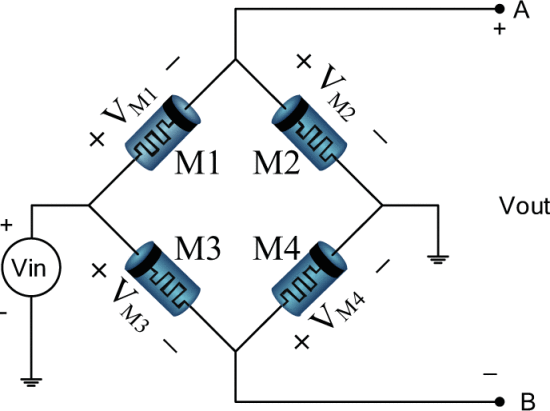
\includegraphics[width=0.25\textwidth]{resources/memristor.png}
        \caption{Building block to a single neuron consisting of 4 memristors as proposed in \cite[Fig.~1]{adhikari2012memristor}}
        \label{fig:memristor}
    \end{figure}

    %TODO: Add fig. 1 aus adhikari2012memristor
    In \ref{fig:memristor} a circuit consisting of 4 identical memristors capable of scaling the input by a specific factor is illustrated.
    The synaptic output can be modeled as the between input voltage $V_{in}$ and the synaptic weight.

    \[V_{out} = \psi \times V_{in}\]

    where $\psi$ can be dynamicially set using the memristors \cite{adhikari2012memristor}.

    \[\psi = \left(\frac{M_2}{M_1+M_1} - \frac{M_4}{M_3+M_4}\right)\]

    This allows for nonvolatile weight storage with comparatively simple hardware.
    It is capable of replacing both digital weight storage and analog weight multiplication.
    

    \section*{Acknowledgment}



    \medskip

    \bibliographystyle{unsrt}
    \bibliography{citations}


\end{document}


